\documentclass[12pt]{article}
\usepackage[margin=0pt, top=1cm, total={14in, 8in}]{geometry}
\usepackage{amsfonts}
\usepackage{amsmath,amssymb,trimclip,adjustbox}
\usepackage{breqn}
\usepackage{hyperref}
\usepackage{tabularray}
\usepackage{flafter} 
\usepackage{tabularx}
\usepackage[dvipsnames]{xcolor} 
\usepackage{polski}
\usepackage[utf8]{inputenc}

\setlength{\parindent}{0pt}
\setlength{\textheight}{720pt}
\setlength{\oddsidemargin}{0pt}
\setlength{\textwidth}{480pt}


\author{Michał Puchyr}
\title{Matematyka dyskretna - notatki na kolokwium 1}

\begin{document}
\maketitle

\section{Multizbiory}

$ X \subseteq Y $ - zawieranie, zbiór $X$ zawiera się lub jest równy zbiorowi $Y$.
Dosłownie każdy element $X$ jest w $Y$.

$ X \subset Y $ - zawieranie właściwe, zbiór $X$ zawiera się w $Y$ oraz $Y$ posiada jakiś element
który nie należy do $X$.

Dla dowolnych zbiorów $A, B, C$:
\begin{itemize}
    \item $\emptyset \subseteq A$
    \item jeżeli $ A \subseteq B $ i $ B \subseteq C $, to $ A \subseteq C $
\end{itemize}

\subsection{Zbiór potęgowy}
Przykład
$$ 2^{\{1, 2, 3\}} = \{\emptyset, \{1\}, \{2\}, \{3\}, \{1,2\}, \{1,3\}, \{2,3\}, \{1,2,3\}\} $$
$$ 2^{\emptyset} = \{ \emptyset \} $$

\subsection{Multizbiór}

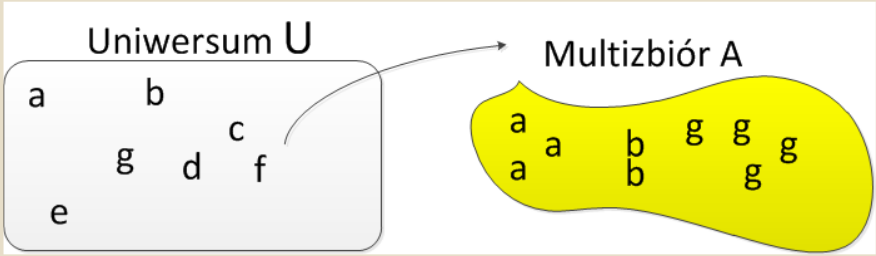
\includegraphics[scale=0.5]{img/multizbior.png}

$$ U = \{a, b, c, d, e, f, g\} \quad A=\{a, a, a, b, b, g, g, g, g\} $$

\begin{table}[!ht]
    \centering
    \caption{Funkcja charakterystyczna multizbioru $ f_a : U \to \{0, 1, ...\} $}
    \begin{adjustbox}{width=0.5\textwidth}
    \begin{tabular}{|c|c|c|c|c|c|c|c|}
        \hline
        x & a & b & c & d & e & f & g \\ \hline
        $f_a(x)$ & 3 & 2 & 0 & 0 & 0 & 0 & 4 \\ \hline
    \end{tabular}
\end{adjustbox}
\end{table}

$$ A=\{(x,fA(x)): x\in U\} A= \{(a,3), (b,2), (c,0), (d,0), (e,0), (f,0), (g,4)\} $$ 

\textbf{Iloczyn}

$$ A \cap B = \{ \ (x,f_{A \cap B} (x)): x \in U \ \textrm{i} \ f_{A \cap B}(x)=min(f_A(x), f_B(x)) \ \} $$

\textbf{Suma}

$$ A \cup B = \{ \ (x,f_{A \cup B} (x)): x \in U \ \textrm{i} \ f_{A \cup B}(x)=max(f_A(x), f_B(x)) \ \} $$

\textbf{Przykład}

$ A=\{\ (a,3), (b,2), (c,0), (d,0), (e,4)\} = \{3a,2b,4e\ \} $

$ B=\{\ (a,0), (b,3), (c,1), (d,2), (e,0)\} = \{3b,c,2d\ \} $ \\

$ A \cap B = \{ \ (a,min(3,0)), (b,min(2,3)), (c,min(0,1)), (d,min(0,2)), (e,min(4,0))\} \\ = \{ \ (a,0),(b,2), (c,0), (d,0), (e,0) \ \} $ \\

$ A \cup B = \{ \ (a,3), (b,3), (c,1), (d,2), (e,4) \ \} $

\section{Rachunek Gentzena}

\subsection{Wzory}

\begin{tabularx}{\textwidth}{X X X X}
    \centering
    $ \displaystyle\frac{\phi \rightarrow \neg \alpha ,\psi }{\phi, \alpha \rightarrow \psi} $ & 
    $ \displaystyle\frac{\phi \rightarrow \alpha \lor \beta, \psi }{\phi \rightarrow \alpha, \beta, \psi} $ &
    $ \displaystyle\frac{\phi \rightarrow \alpha \land \beta, \psi }{\phi, \alpha \rightarrow \psi || \phi, \beta \rightarrow \psi} $ &
    $ \displaystyle\frac{\phi \rightarrow \alpha, \alpha \psi}{\phi \rightarrow \alpha, \psi} $ \\[20pt]

    \centering
    $ \displaystyle\frac{\phi, \neg \alpha \rightarrow \psi}{\phi \rightarrow \alpha, \psi} $ &
    $ \displaystyle\frac{\phi, \alpha \lor \beta \rightarrow \psi}{\phi, \alpha \rightarrow \psi || \phi, \beta \rightarrow \psi} $ &
    $ \displaystyle\frac{\phi, \alpha \land \beta \rightarrow \psi}{\phi, \alpha, \beta \rightarrow \psi} $ & 
    $ \displaystyle\frac{\phi, \alpha, \alpha \rightarrow \psi}{\phi, \alpha \rightarrow \psi} $ \\[20pt]
\end{tabularx}

$ P_1 : (\alpha \Rightarrow \beta) \Leftrightarrow (\neg \alpha \lor \beta) \quad \quad 
P_2 : (\alpha \Leftrightarrow \beta) \Leftrightarrow ((\alpha \Rightarrow \beta) \land (\beta \Rightarrow \alpha)) $

\section{Relacje binarne}

\begin{table}[h]
    \centering
    \begin{tabular}{|c|c|c|c|}
    \hline
    $R_2$ & a & b & c \\ \hline
    a & 1 & 1 & 0 \\ \hline
    b & 0 & 0 & 0 \\ \hline
    c & 0 & 0 & 0 \\ \hline
    \end{tabular}
\end{table}

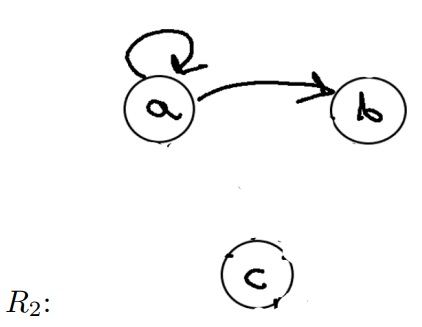
\includegraphics[scale=0.5]{img/grafR2.png}

\subsection{Własności relacji}

Niech dana będzie relacja binarna na $ R \subseteq X \times X $

Za przykładowe uniwersum posłuży nam zbiór $U = \{ a, b, c, d \} $ \\

Własności relacji i ich warunki

\begin{itemize}
    \item Zwrotna -- $\forall x \in X (<x,x> \in R)$
    
    Aby było zwrotna w relacji \textbf{musi} znaleźć się $ \{ <a, a>, <b, b>, <c, c>, <d, d> \} $

    \item Przeciwsymetryczna -- $\forall x \in X(\neg <x, x> \in R) $
    
    Aby była przeciwzwrotna to w relacji \textbf{nie może} znaleźć się \textbf{żadna} z tych par \linebreak 
    $ <a, a>, <b,b>, <c,c>, <d,d> $
    
    \item Symetryczna -- $ \forall x, y \in X(<x,y> \in R \Rightarrow <y,x> \in R) $
    
    Aby była symetryczna to \textbf{każda istniejąca para w relacji} musi mieć swoje lustrzane odbicie. Na przykład:
    $ \{ <a,b>, <b,a>, <a, a>, <b,c>, <c,b> \} $

    \item Asymetryczna -- $\forall x,y \in X((<x,y> \in R \land (y,x) \in R) \Rightarrow x=y) $
    
    \item Przeciwsymetryczna -- $\forall x,y \in X(<x,y> \in R) \Rightarrow \neg <y,x> \in R) $
\end{itemize}

\section{Podobieństwo zbiorów klasycznych}

Przyjmijmy, że:

$ a = |X\cap Y| $

$ b = |X\backslash Y| $

$ c = |Y\backslash X| $

$ d = |\overline{X} \cap \overline{Y}| $ \\

\subsection*{Typ 1 współczynników podobieństwa zbiorów}

Jaccard: $ P_{Jac}(X,Y) = \dfrac{|X \cap Y|}{|X \cup Y|} = \dfrac{a}{a+b+c} $

Dice: $ P_{Dic}(X,Y) = \dfrac{|X \cap Y|}{|X| + |Y|} = \dfrac{a}{2a+b+c} $

Dice 2: $ P_{2Dic}(X,Y) = \frac{2|X \cap Y|}{|X| + |Y|} = \dfrac{2a}{2a+b+c} $

Overlap: $ P_{Overlap}(X,Y) = \dfrac{|X \cap Y|}{\min\{|X|, |Y|\}}$

Cosinus: $ P_{Cosinus}(X,Y) = \dfrac{|X \cap Y|}{\sqrt{|X|} \cdot \sqrt{|Y|}}$

Sorensen: $ P_{Sor}(X,Y) = \dfrac{4a}{4a + b + c} $

Anderberg: $ P_{And}(X,Y) = \dfrac{8a}{8a + b + c} $

Sneath i Sokal 2: $ P_{SS2} = \dfrac{a}{a + 2(b+c)} $

Ochiai: $ P_{Och} = \dfrac{a}{\sqrt{a+b} \cdot \sqrt{b+c}} $

Kulczyński 2: $ P_{Ku2} = \dfrac{1}{2} \left( \dfrac{a}{a+b} + \dfrac{a}{a+c} \right) $

Tversky : $ P_{Tve} = \dfrac{a}{a + \alpha \cdot b + \beta \cdot c} $, przy założeniu $ \alpha, \beta > 0 $

\subsection*{Typ 2 współczynników podobieństwa zbiorów}

Rogers i Tamimoto: $ P_{RT}(X,Y) = \dfrac{a+d}{a + 2(b+c) + d} $

Sokal i Michener: $ P_{SM}(X,Y) = \dfrac{a+b}{a + b + c + d} $

Sneath i Sokal 1: $ P_{SS1}(X,Y) = \dfrac{a+b}{a + \frac{1}{2}(b + c) + d} $

Russel i Rao: $ P_{RR}(X,Y) = \dfrac{a}{a+b+c+d} $

Yule i Kendall: $ P_{YUK}(X,Y) = \dfrac{a \cdot d}{a \cdot d + b \cdot c} $

\subsection*{Odległość zbiorów klasycznych}

\textbf{Liczność różnicy symetrycznej}: $d_{SYM}(X, Y ) = card(X \backslash Y ) + card(Y \backslash X) = b + c$
(określana także innymi nazwami np. City-block distance, Manhattan distance, Hamming distance.) \\

\textbf{Odległość Euklidesowa:}

$d_{Euc}(X,Y) = \sqrt{\sum_{i=1}^{n} (u_X(u_i) - u_Y(u_i))^2} = \sqrt{b+c} $, \ gdzie $u_X$ i $u_Y$ są funkcjami charakterystycznymi
odpowiednio zbiorów $X$ i $Y$.

\section{Pomocne}

\begin{itemize}
    \item Ile jest relacji dla $ |U| = 5 $? Odpowiedź : $ 2^{25} $
\end{itemize}

\subsection{Jak rozróżnić należenie od zawierania}

\begin{itemize}
    \item $ A = \{ \emptyset \} $ \ i \ $ B = \{ \emptyset, \{ \emptyset \} \} $ -- $ A \in B \quad A \subseteq B$
    \item $ A = \{ \emptyset \} $ \ i \ $ B = \{\{\emptyset\}\}$ -- $ A \in B \quad A \nsubseteq B $
    \item $ A = \{ \emptyset \} $ \ i \ $ B = \{ \emptyset, \{ \{ \emptyset \} \} \} $ -- $ A \notin B \quad A \subseteq B $
    \item $ A = \{ \emptyset \} $ \ i \ $ B = \{\{\{ \emptyset \}\}\} $ -- $ A \notin B \quad A \nsubseteq B $
\end{itemize}

\subsection{Zbiór potęgowy oraz jego prawdy}

\begin{itemize}
    \item $ \emptyset \in 2^{\emptyset} $ -- \textcolor{Green}{Prawda}
    \item $ \emptyset \subseteq 2^{\emptyset} $ -- \textcolor{Green}{Prawda}
    \item $ \emptyset \subset 2^{\emptyset} $ -- \textcolor{red}{Fałsz}
\end{itemize}

\end{document}